\section{Evaluation}
\label{sec:evaluation}

This section demonstrates performance improvements brought by our GPU
implementations for the existing vehicle detection program
\cite{Niknejad12}.
We also discuss the details of performance comparisons among our GPU
implementations and traditional CPU implementations identifying the
fundamental factors that allow GPUs to outperform CPUs.

\subsection{Experimental Setup}
\label{sec:setup}

We prepare three variants of the vehicle detection program implemented
using (i) a single CPU core, (ii) multiple CPU cores, (iii) and
massively parallel GPU compute cores.
The CPU implementations use the Intel Core i7 3930K (@3.2GHz) and the
Xeon E5-2643 (@3.3GHz) series while we provide several different GPUs
for the GPU implementations: namely NVIDIA GeForce GTX 560 Ti, GTX 580,
GTX 680, GTX TITAN, and Tesla K20Xm.
The same set of 10 images as previous work \cite{Niknejad12} is used as
input data and their average execution time is considered as major
performance metrics.
Note that this execution time includes all relevant pieces of image
processing such as image loading and output rendering in addition to the
primary object detection block.

\subsection{Experimental Results}
\label{sec:results}

\begin{figure}[t]
 \begin{center}
  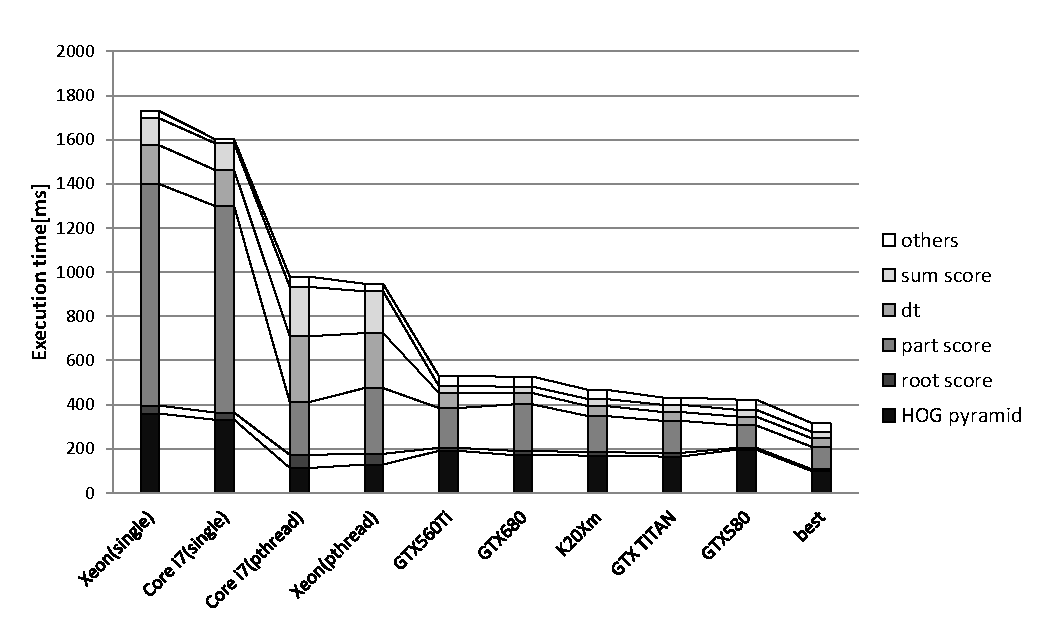
\includegraphics[width=\hsize]{fig/float_exe_time.eps}\\
  \caption{Execution times of the single-precision floating-point program.}
  \label{fig:float_exe_time}
 \end{center}
\end{figure}

\begin{figure}[t]
 \begin{center}
  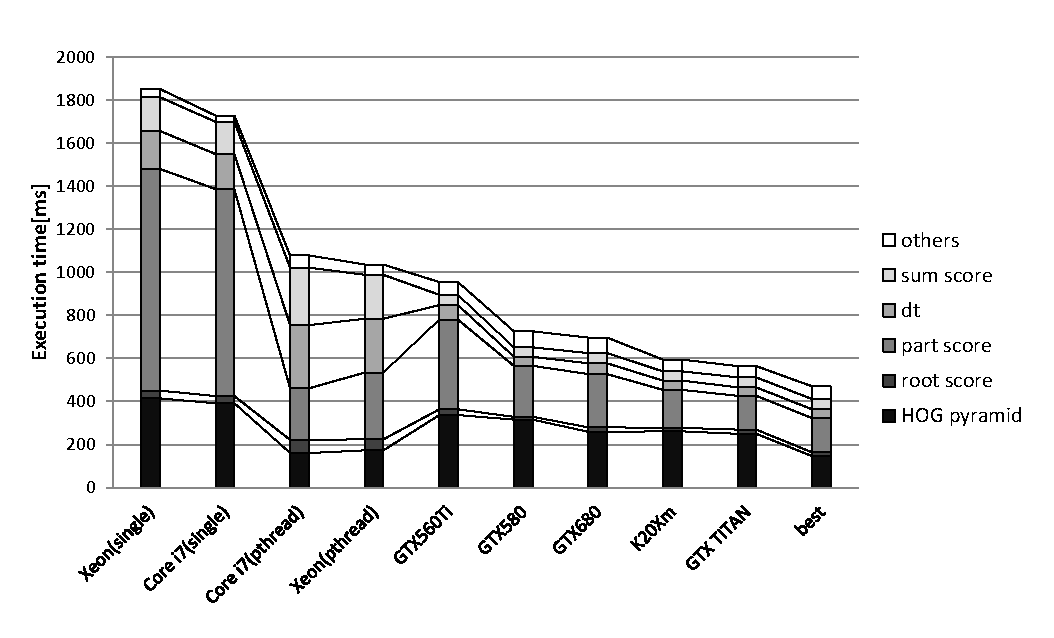
\includegraphics[width=\hsize]{fig/double_exe_time.eps}\\
  \caption{Execution times of the double-precision floating-point program.}
  \label{fig:double_exe_time}
 \end{center}
\end{figure}

Fig.~\ref{fig:float_exe_time} shows the execution times of all variants
of the vehicle detection program configured to use single-precision
floating-point operations.
The dimensions of input images are 640$\times$480 pixels.
``XXX(single)'' uses a single CPU core for the corresponding CPU series
while ``XXX(multicore)'' uses multiple CPU cores with \textit{pthread}.
Other labels except for ``best'' represent our GPU implementations using
the corresponding GPUs; ``best'' describes the best combination of the
GPU and CPU implementations.
For the GPU implementations, we shape each CUDA block by $8 \times 8$
threads.
It is notable to see that most computational blocks benefit from GPUs
but only the HOG calculation prefers the multicore implementation.
This is attributed to the fact that the HOG calculation contains atomic
operations as illustrated in Listing~\ref{lst:hog} that could squeeze
massively parallel threads of the GPU.

Comparisons among the GPUs as well as those among the CPUs provide an
intriguing observation.
The GPUs based on the state-of-the-art \textit{Kepler}
architecture \cite{NVIDIA_Kepler} are inferior to those based on the
old \textit{Fermi} architecture \cite{NVIDIA_Fermi}.
Albeit a significant number of compute cores with the enhanced
multithreading mechanism, the Kepler GPUs operate at lower frequency
than the Fermi GPUs due to their complex architecture.
Since the vehicle detection program employs a lot of compute-intensive
blocks as depicted through Listing~\ref{lst:score} to \ref{lst:hog}, the
operating  frequency is more dominating than the architectural benefit.
This is a useful finding toward the future development of GPU-based
image processing.
It is also remarkable that the Core i7 CPU is slightly faster than the
Xeon CPU.
Since the experiment is limited to a single process, we suspect that a
desktop-oriented design of the Core i7 CPU is preferred to a
server-oriented design of the Xeon CPU.

As a whole, the best performance is obtained from such a setup that
uses the multicore implementation for the HOG calculation while
offloading other computational blocks to the GeForce GTX 580 GPU.
It results in a speed-up of more than 3x to 5x for the execution of
vehicle detection over the traditional single-core CPU implementation
and the multicore CPU implementation respectively.
This scale of speed-up for the overall execution of a complex real-world
application is a significant contribution, whereas an order-of-magnitude
speed-up has been reported for particular blocks of the program and the
algorithm in previous work \cite{Chen11, Prisacariu09}.
Our results truly demonstrate the current performance status of
state-of-the-art GPUs for practical vehicle detection.

Fig. \ref{fig:double_exe_time} shows the execution times of all variants
of the vehicle detection problem configured to use double-precision
floating-point operations.
Unlike the single-precision scenario, the Kepler GPUs outperform the
Fermi GPUs.
This explains that the double-precision performance of GPUs is improved
as the generation of GPUs advances.
Another notable finding is that the TITAN GPU is slightly faster than
the K20Xm GPU for our vehicle detection program.
This is due to a slightly higher operating frequency of the TITAN GPU.
Since the TITAN GPU is a consumer market price while the K20Xm is a very
expensive supercomputing device, we suggest that the vehicle detection
program uses the TITAN GPU for a better cost performance.

Henceforth we restrict our attention to the single-precision
floating-point version of the vehicle detection program.
Note that similar performance characteristics were also observed in the
double-precision version through our experiments but they are omitted
herein due to a space constraint.

\begin{figure}[t]
 \begin{center}
  \includegraphics[width=\hsize]{fig/time_on_image_size.eps}\\
  \caption{Impact of the image size on execution times.}
  \label{fig:time_on_image_size}
 \end{center}
\end{figure}

Fig. \ref{fig:time_on_image_size} shows the impact of the image size on
execution times. 
The GPU implementation uses the GeForce GTX 580 GPU, which is the best
performer in all the GPUs demonstrated in Fig. \ref{fig:float_exe_time}.
The lessons learned from this experiment are that the execution time of
the vehicle detection program is proportionally influenced by the input
image size.
Therefore the benefit of our GPU implementations as compared to the
traditional CPU implementations would hold for more high-resolution
image processing.

\begin{figure}[t]
 \begin{center}
  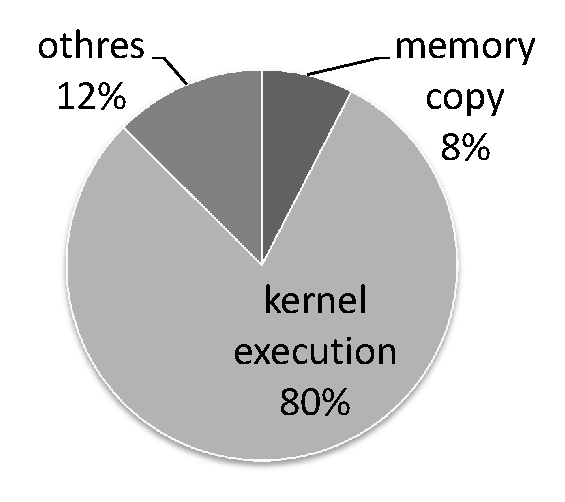
\includegraphics[width=0.49\hsize]{fig/breakdown_gpu.eps}\\
  \caption{The breakdown of execution times of the GPU implementation.}
  \label{fig:breakdown_gpu}
 \end{center}
\end{figure}

Fig. \ref{fig:breakdown_gpu} shows the breakdown of execution times of
the GPU implementation that achieves the best performance for the
vehicle detection program.
The memory copy overhead is often claimed to be a bottleneck in GPU
programming \cite{Jablin_PLDI11}, but our analysis explains that it is
not the case for the exhibited workload.
This means that further advances of GPU technology will lead to faster
implementations of the vehicle detection program, which encourages
future work to use state-of-the-art GPUs.

\begin{figure}[t]
 \begin{center}
  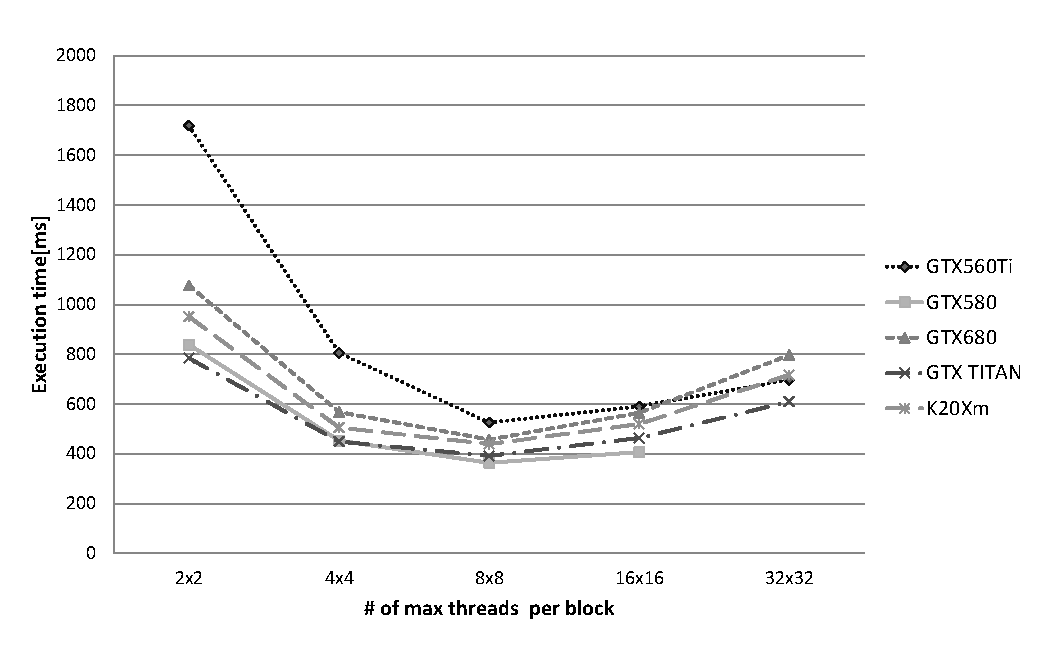
\includegraphics[width=\hsize]{fig/impact_of_blockshape.eps}\\
  \caption{Impact of the block shape on execution times.}
  \label{fig:impact_of_blockshape}
 \end{center}
\end{figure}

Fig. \ref{fig:impact_of_blockshape} shows the impact of the block shape
of GPU code on the execution times of the single-precision
floating-point vehicle detection program.
Particularly the number of threads in each block is varied to see how
the performance is affected.
Note that the Fermi GPUs cannot support 32$\times$32 threads per block
due to the hardware limitation.
From what we observed in our experiment, a configuration of 8$\times$8
threads exhibits the best performance for all the GPUs.
This is somewhat an intuitive expectation because each warp of the GPU
can contain up to 32 threads and a set of two warps is executed every
two cycles according to the NVIDIA GPU architecture.
Having less threads per block looses parallelism while introducing more
threads could cause resource conflict within a block.
Therefore a more in-depth investigation is required to truly optimize
performance.
